\documentclass[11pt,a4paper]{article}

\usepackage[T1]{fontenc}
\usepackage[utf8]{inputenc}
\usepackage{lmodern}
\usepackage[margin=2.4cm]{geometry}
\usepackage{amsmath,amssymb}
\usepackage{booktabs,tabularx,longtable,array}
\usepackage{xcolor}
\usepackage{listings}
\usepackage{graphicx}
\usepackage{float}
\usepackage{enumitem}
\usepackage{tikz}
\usetikzlibrary{arrows.meta,positioning,shapes.geometric,fit}
\usepackage[colorlinks=true,linkcolor=blue!50!black,urlcolor=blue!50!black,citecolor=blue!50!black]{hyperref}

\definecolor{codebg}{RGB}{247,247,247}
\definecolor{codekw}{RGB}{0,0,150}
\definecolor{codecm}{RGB}{90,120,90}
\definecolor{codestr}{RGB}{160,40,40}
\definecolor{addcol}{RGB}{0,110,0}
\definecolor{delcol}{RGB}{170,0,0}

\lstdefinestyle{c}{
  language=C, basicstyle=\ttfamily\footnotesize, backgroundcolor=\color{codebg},
  keywordstyle=\color{codekw}\bfseries, commentstyle=\color{codecm}\itshape,
  stringstyle=\color{codestr}, showstringspaces=false, breaklines=true,
  frame=single, rulecolor=\color{black!20}, columns=fullflexible,
  morekeywords={real,complex,BOOLEAN,bool,integer}}
\lstdefinestyle{diff}{
  basicstyle=\ttfamily\footnotesize, backgroundcolor=\color{codebg},
  breaklines=true, frame=single, rulecolor=\color{black!20}, columns=fullflexible,
  moredelim=**[il][\color{addcol}]{+},
  moredelim=**[il][\color{delcol}]{-}}
\lstdefinestyle{sh}{
  basicstyle=\ttfamily\footnotesize, backgroundcolor=\color{codebg},
  breaklines=true, frame=single, rulecolor=\color{black!20}, columns=fixed,
  basewidth=0.5em, keepspaces=true}
\lstset{style=c}
\sloppy
\setlength{\emergencystretch}{3em}

\newcommand{\file}[1]{\texttt{#1}}
\newcommand{\fn}[1]{\texttt{#1()}}
\newcommand{\var}[1]{\texttt{#1}}
\newcommand{\opt}[1]{\texttt{#1}}
\newcommand{\Hsoc}{H_{\mathrm{SOC}}}

\title{\textbf{Advances in YAeHMOP}\\[4pt]
\Large Spin polarization and spin--orbit coupling in the \texttt{tightbind} program\\[4pt]
\large Developer notes for the \texttt{adias-dev} branch of the fork \texttt{ac-dias/yaehmop}}
\author{Alexandre C. Dias\\(prepared with the help of Claude, Anthropic)}
\date{November 2026}

\begin{document}
\maketitle

\begin{abstract}
This document describes, file by file, every change made to the \texttt{tightbind}
program of YAeHMOP in the fork \url{https://github.com/ac-dias/yaehmop} (branch
\texttt{adias-dev}) since upstream commit \texttt{4ded45b} (``bump min cmake version
to 10''). The changes add (i)~spin-polarized calculations with one parameter table per
spin channel, (ii)~on-site spin--orbit coupling (SOC) in a spinor basis, (iii)~a
configurable Wolfsberg--Helmholz constant for the diagonal $H_{ii}(\mathbf{k})$ term, which
was hardwired to $1.75$, and (iv)~two small fixes. Runs without the new options give
byte-identical output to the original program. The aim of these notes is to make the
review of a pull request to \url{https://github.com/greglandrum/yaehmop} easy: each
change is explained, motivated, shown as code and tied to a test. Section~\ref{sec:inputs}
summarizes what changed for the user (command line, input keywords, new input and
output files), and Section~\ref{sec:examples} closes with two worked examples, MoS$_2$ with
SOC and ferromagnetic bcc Fe, run with the new code.
\end{abstract}

\tableofcontents
\newpage

%=====================================================================
\section{Summary of the changes}
%=====================================================================

\subsection{What the new features do}

\begin{description}[style=nextline,leftmargin=1.2em]
\item[Spin-polarized runs (\opt{--parm-up}, \opt{--parm-down})]
Each spin channel is an independent extended Hückel calculation that uses its own parameter
table, so the channels can have different $H_{ii}$ and zetas. The two channels run in two
child processes at the same time. Their outputs carry the suffix \texttt{\_up} or
\texttt{\_down}. Each channel holds one electron per state. The electron count of each
channel and its Wolfsberg--Helmholz constant can be set on the command line
(\opt{--nelec-up}, \opt{--nelec-down}, \opt{--const-up}, \opt{--const-down}).

\item[Spin--orbit coupling (\opt{--soc})]
An on-site $\lambda_{A,l}\,\mathbf{L}\cdot\mathbf{S}$ term is added to the spinless
$H(\mathbf{k})$ in a basis of $2n$ spinors. The program writes $2n$ bands, the Fermi level
and total DOS with one electron per state, and the spinor $H(\mathbf{k})$, $S(\mathbf{k})$
in the usual \texttt{.HAM}/\texttt{.OV} binary format, plus a text file with $\Hsoc$.

\item[\texttt{THE CONST DIAG}]
A new input keyword for the $K$ of the term that couples an orbital with its own images in
the other cells. The original code always used $K=1.75$ for this term
(\file{K\_hamil.c}), whatever \texttt{THE CONST} said. The default stays $1.75$.

\item[Fixes]
\texttt{.HAM} is now truncated when it is opened. Before, running twice in the same
directory appended to the old file. In THIN mode the off-diagonal $H(\mathbf{k})$
elements now use \texttt{THE CONST}; $1.75$ was hardwired there too.
\end{description}

\subsection{Files at a glance}

\begin{longtable}{>{\ttfamily\small\raggedright}p{4.7cm} c p{8.4cm}}
\toprule
\textrm{\textbf{file}} & \textbf{status} & \textbf{what changed} \\
\midrule
\endhead
tightbind/soc.c        & new      & the whole SOC implementation (reading $\lambda$, $\mathbf{L}$ matrices, spinor matrices, diagonalization, dumps, Fermi level/DOS) \\
tightbind/main.c       & modified & new command-line parser; one process per spin channel \\
tightbind/driver.c     & modified & \fn{run\_bind\_ex} (input name $\neq$ output name); channel set-up; calls to the SOC code \\
tightbind/kpoints.c    & modified & SOC branch in the $k$-point loop; \texttt{O\_TRUNC} for \texttt{.HAM} \\
tightbind/bands.c      & modified & SOC branch in the band structure ($2n$ bands) \\
tightbind/K\_hamil.c   & modified & \var{details->the\_const\_diag} instead of the hardwired \var{THE\_CONST} \\
tightbind/fileio.c     & modified & parsing of \texttt{THE CONST DIAG} \\
tightbind/bind.h       & modified & new field \var{the\_const\_diag}; new globals; macro \var{VALENCE\_FRACTION} \\
tightbind/globals.c    & modified & definitions of the new globals \\
tightbind/prototypes.h & modified & prototypes of \fn{run\_bind\_ex} and of the \file{soc.c} functions \\
tightbind/mulliken.c   & modified & occupation \var{max\_occup} instead of 2; valence fraction in the net charges \\
tightbind/avg\_props.c & modified & same, for the crystal occupations and average net charges \\
tightbind/DOS\_stuff.c & modified & ``states are present'' counts use \var{max\_occup} \\
tightbind/genutil.c    & modified & electron-count sanity check uses \var{max\_occup} \\
tightbind/CMakeLists.txt,\newline tightbind/Makefile,\newline tightbind/makefile.linux & modified & \file{soc.c} added to the sources \\
docs/SPIN\_SOC.md      & new      & user documentation of the new options \\
tests/spin\_soc/       & new      & automated tests (\file{run\_tests.py}) and their data \\
examples/spin\_soc/,\newline new\_tests/ & new & small examples; band structures of MoS$_2$ (SOC) and bcc Fe (spin) with outputs and figures \\
README.md, .gitignore  & modified & short section on the fork; ignore Python caches \\
\bottomrule
\end{longtable}

In numbers, for the code, tests and examples: about 1\,500 lines added and 50 removed in
28 files; about 540 of the added lines are \file{soc.c} and 356 are the test script. The core numerical routines (overlaps, $H(R)$,
Bloch sums, symmetry, properties) are not touched.

\subsection{Commits on the branch}
\begin{center}
\begin{tabular}{>{\ttfamily}l p{11.5cm}}
\toprule
866e130 & spin polarization (one table per channel) and SOC in the tightbinding program; \texttt{.HAM} truncation fix; docs, example and tests \\
c38236f & configurable $K$ (\texttt{THE CONST DIAG}, \opt{--const-up/--const-down}); \texttt{new\_tests} \\
722ba73 & remove a \texttt{\_\_pycache\_\_} committed by mistake; \file{.gitignore} \\
\bottomrule
\end{tabular}
\end{center}

%=====================================================================
\section{What changed in the inputs (and outputs)}\label{sec:inputs}
%=====================================================================

This section is the user's view of the changes. Everything here is optional: an input
file and a command line that work with the original program work unchanged and give the
same results.

\subsection{Command line}

The original program accepted \texttt{bind <input> [paramfile]},
\texttt{bind --use\_stdin\_stdout [paramfile]} and \texttt{bind -v}. These forms are
unchanged. Options starting with \texttt{--} can now be given before the input file:

\begin{lstlisting}[style=sh]
bind [options] <inputfile> [paramfile]
bind --use_stdin_stdout [paramfile]

  --parm-up FILE --parm-down FILE  spin-polarized run: one parameter table per spin
                    channel; outputs get _up / _down before the input extension
                    (one electron per state in each channel)
  --nelec-up X --nelec-down X      electrons in each channel (default: half of the
                    electrons of the input in each one)
  --const-up K --const-down K      Wolfsberg-Helmholz K of each channel
                    (default: THE CONST of the input)
  --soc FILE        spin-orbit coupling, lines 'Element shell lambda(eV)'
  -v                print the version
  -h, --help        print this list
\end{lstlisting}

\begin{center}
\begin{tabularx}{\textwidth}{>{\ttfamily}l X}
\toprule
\textrm{\textbf{option}} & \textbf{rules} \\
\midrule
--parm-up/--parm-down & both or none; not with \texttt{--use\_stdin\_stdout}; the
  tables replace the second positional argument (giving both is an error) \\
--nelec-*, --const-* & only with \texttt{--parm-up/--parm-down}; each one is optional \\
--soc & works with the usual \texttt{[paramfile]}; not with spin polarization (yet);
  needs a LAPACK build \\
unknown \texttt{--}option & stops with the usage message \\
\bottomrule
\end{tabularx}
\end{center}

\subsection{Input file (\texttt{.bind})}

There is one new keyword. Every other keyword keeps its syntax and meaning.

\begin{center}
\begin{tabularx}{\textwidth}{>{\ttfamily}l X}
\toprule
\textrm{\textbf{keyword}} & \textbf{meaning} \\
\midrule
THE CONST DIAG <K> & $K$ of the diagonal $H_{ii}(\mathbf{k})$ term (an orbital with its
  own images in the other cells). Default 1.75, which is what the original program
  always used. The value can be on the same line or on the next one, like
  \texttt{THE CONST}. See Section~\ref{sec:kdiag}. \\
\bottomrule
\end{tabularx}
\end{center}

Some existing keywords are interpreted differently in the new modes:
\begin{itemize}
\item \texttt{Electrons} / \texttt{Charge}: in a spin-polarized run they give the total for
  both channels. Each channel gets half, unless \opt{--nelec-up/--nelec-down} are given.
  With SOC they give the number of electrons in the $2n$ spinor states (one per state).
\item \texttt{THE CONST}: in a spin-polarized run it is replaced in each channel by
  \opt{--const-up/--const-down} when those are given.
\item \texttt{Dump Hamil} / \texttt{Dump Overlap}: in a spin-polarized run each channel
  writes its own files. With SOC the files hold the $2n\times2n$ spinor matrices.
\item Keywords for properties that are not implemented with SOC (projected DOS, COOP,
  FMO, populations, charge iteration, Walsh, MO and matrix printing, \ldots) stop a SOC run
  with a message naming the keyword. Charge iteration also stops a spin-polarized run.
\end{itemize}

\subsection{Parameter tables}

The format of the parameter tables (\file{eht\_parms.dat}) is unchanged. In a
spin-polarized run there are two of them, one per channel. They must contain the same
elements and shells, but any value can differ ($H_{ii}$, zetas, double-zeta
coefficients).

\subsection{New input file: SOC constants}

\opt{--soc FILE} reads one line per element and shell, with $\lambda$ in eV. Lines starting
with \texttt{\#}, \texttt{;} or \texttt{!} are comments, symbols are case-insensitive, and
shells are $p$, $d$ or $f$ ($s$ lines are ignored with a message):
\begin{lstlisting}[style=sh]
# element shell lambda_eV
Mo  d  0.063352
S   p  0.197577
\end{lstlisting}
This is the same format as the \file{soc\_parameters.txt} written by yaehmop-bandfit.

\subsection{Outputs}

\begin{center}
\begin{tabularx}{\textwidth}{l X}
\toprule
\textbf{mode} & \textbf{outputs} \\
\midrule
spin polarized & every output twice, with \texttt{\_up}/\texttt{\_down} inserted before
  the extension of the input name: \texttt{MoS2.bind} $\to$
  \texttt{MoS2\_up.bind.out}, \texttt{MoS2\_down.bind.band}, \ldots; formats unchanged \\
SOC & \texttt{.band} with $2n$ energies per $k$ point (header ``\texttt{2n orbitals in the
  unit cell.}''); \texttt{.HAM}/\texttt{.OV} with $2n\times2n$ spinor matrices in the
  usual binary format (Eq.~\eqref{eq:packed}; orbitals $1..n$ spin up, $n+1..2n$ spin
  down); new text file \texttt{.SOC} with the nonzero elements \texttt{i j Re Im} of
  $\Hsoc$ \\
\bottomrule
\end{tabularx}
\end{center}

New keys in the \texttt{.out}: \texttt{\#SPIN\_CHANNEL}, \texttt{\#ELECTRONS\_THIS\_CHANNEL}
and \texttt{\#THE\_CONST} in spin-polarized runs; \texttt{\#SOC\_STATES} and the list of
$\lambda$ used per atom with SOC; \texttt{\#THE\_CONST\_DIAG} when it is not the default.
They start with \texttt{\#} or \texttt{;}, like the existing ones.

%=====================================================================
\section{Background: the parts of the program that matter here}
%=====================================================================

This section recalls the pieces of the existing code that the new features build on,
so that the later sections can refer to them.

\subsection{Control flow}

Figure~\ref{fig:flow} shows the path from \fn{main} to the outputs. The new code hooks
in at four places, marked in color: the argument parser in \fn{main}, the set-up in
\fn{run\_bind\_ex}, the $k$-point loop, and the band-structure loop.

\begin{figure}[ht]
\centering
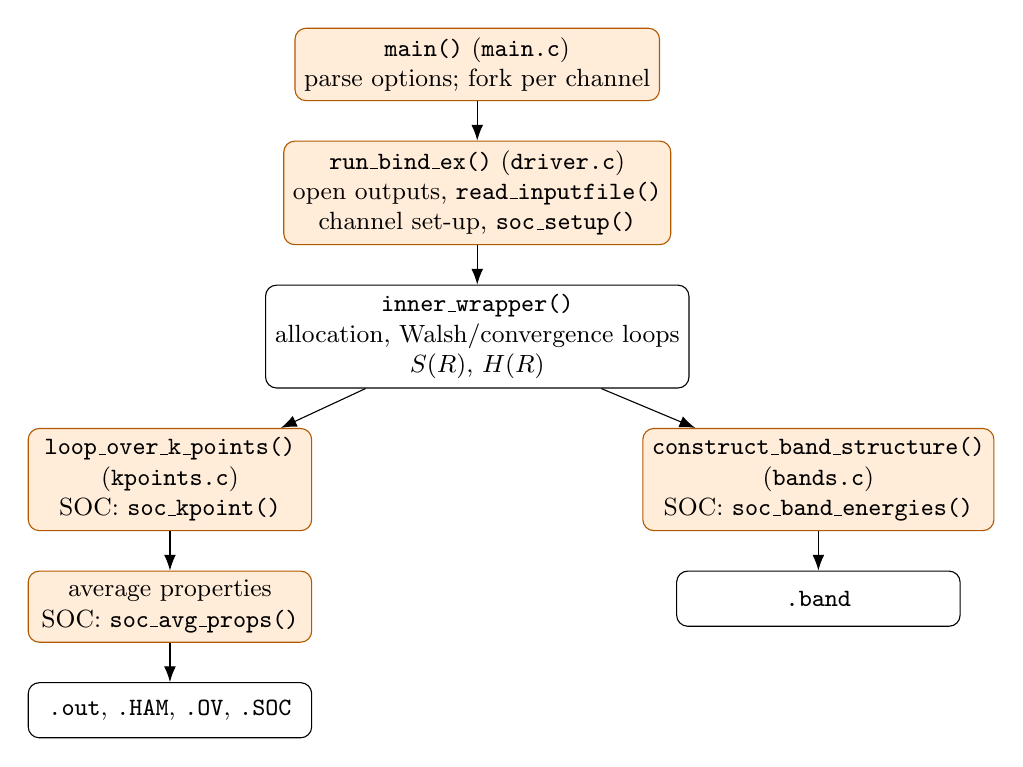
\begin{tikzpicture}[node distance=5mm and 8mm,
  box/.style={draw,rounded corners,align=center,font=\small,minimum width=3.6cm,minimum height=7mm,fill=white},
  new/.style={box,fill=orange!15,draw=orange!70!black},
  arr/.style={-{Latex[length=2mm]}}]
\node[new] (main) {\texttt{main()} (\file{main.c})\\parse options; fork per channel};
\node[new,below=of main] (run) {\texttt{run\_bind\_ex()} (\file{driver.c})\\open outputs, \texttt{read\_inputfile()}\\channel set-up, \texttt{soc\_setup()}};
\node[box,below=of run] (inner) {\texttt{inner\_wrapper()}\\allocation, Walsh/convergence loops\\$S(R)$, $H(R)$};
\node[new,below left=of inner,xshift=1.4cm] (kloop) {\texttt{loop\_over\_k\_points()}\\(\file{kpoints.c})\\SOC: \texttt{soc\_kpoint()}};
\node[new,below right=of inner,xshift=-1.4cm] (bands) {\texttt{construct\_band\_structure()}\\(\file{bands.c})\\SOC: \texttt{soc\_band\_energies()}};
\node[new,below=of kloop] (avg) {average properties\\SOC: \texttt{soc\_avg\_props()}};
\node[box,below=of bands] (bandout) {\texttt{.band}};
\node[box,below=of avg] (out) {\texttt{.out}, \texttt{.HAM}, \texttt{.OV}, \texttt{.SOC}};
\draw[arr] (main)--(run); \draw[arr] (run)--(inner);
\draw[arr] (inner)--(kloop); \draw[arr] (inner)--(bands);
\draw[arr] (kloop)--(avg); \draw[arr] (avg)--(out); \draw[arr] (bands)--(bandout);
\end{tikzpicture}
\caption{Simplified control flow of \texttt{bind}. Orange boxes contain new or changed code.}
\label{fig:flow}
\end{figure}

\subsection{Storage of Hermitian matrices}\label{sec:packed}

$H(\mathbf{k})$ and $S(\mathbf{k})$ are stored in \var{hermetian\_matrix\_type}: one real
array \var{mat} of $n\times n$ doubles. The real part of element $(i,j)$, $i<j$, is in the
upper triangle, the imaginary part in the lower triangle, and the diagonal is real. Before
LAPACK is called, \file{kpoints.c} and \file{bands.c} copy the array into a complex matrix
like this:
\begin{lstlisting}
cmplx_hamil[j*n+k].r = hamilK.mat[j*n+k];   /* k > j */
cmplx_hamil[j*n+k].i = hamilK.mat[k*n+j];
\end{lstlisting}
and call \texttt{zhegv} with \texttt{uplo='L'}. Because Fortran is column-major, C element
\texttt{[j][k]} is Fortran element $(k,j)$, in the lower triangle. The matrix that LAPACK
diagonalizes therefore has
\begin{equation}
A_{kj} = \texttt{mat}[j][k] + i\,\texttt{mat}[k][j], \qquad k>j ,
\end{equation}
and so the physical matrix (the one whose eigenvalues are computed) is
\begin{equation}\label{eq:packed}
\boxed{\;H_{ij} = \texttt{mat}[i][j] - i\,\texttt{mat}[j][i]\quad (i<j),\qquad H_{ji}=H_{ij}^{*}\;}
\end{equation}
This is also how the binary dumps \texttt{.HAM}/\texttt{.OV} must be read (header
\texttt{int nk, int n}, then one $n\times n$ \texttt{double} array per $k$ point). We
checked against interatomic distances that, read this way, $H(\mathbf{k})=\sum_R
e^{+i\mathbf{k}\cdot\mathbf{R}}H(\mathbf{R})$ with $H_{ij}(\mathbf{R})=\langle\phi_i(0)|H|\phi_j(\mathbf{R})\rangle$.
The SOC code writes its spinor matrices in exactly this layout, so the existing
diagonalization path, the dump format and external readers all keep working.

\subsection{Orbital order}

\fn{build\_orbital\_lookup\_table} (\file{genutil.c}) stores the index of the first
orbital of each atom. Within an atom the order is $s$; $p_x,p_y,p_z$;
$d_{x^2-y^2}, d_{z^2}, d_{xy}, d_{xz}, d_{yz}$; $f_{z^3}, f_{xz^2}, f_{yz^2}, f_{xyz},
f_{z(x^2-y^2)}, f_{x(x^2-3y^2)}, f_{y(3x^2-y^2)}$ (see \fn{map\_orb\_num\_to\_name}).
A shell is present only if its principal quantum number is nonzero. Dummy atoms have
\var{orbital\_lookup\_table[i]} $=-1$.

\subsection{Global state}

The matrices, file pointers, \var{unit\_cell} and \var{details} are globals
(\file{globals.c}), and there are roughly a hundred \texttt{static} variables in the
source (\file{lovlap.c}, \file{diag.c}, \file{electrostat.c}, \ldots). Running two
calculations one after the other in the same process is therefore not safe without a
careful clean-up. This is why the spin channels run in separate processes
(Section~\ref{sec:spin}).

%=====================================================================
\section{Generalized occupation: \texttt{max\_occup} and \texttt{VALENCE\_FRACTION}}\label{sec:occ}
%=====================================================================

Both new features need levels that hold \emph{one} electron instead of two: a spin
channel has one electron per state, and so does a spinor state with SOC. In the original
code the value 2 is written in the occupation routines. We replaced it by a global
\var{max\_occup}. Its default of 2.0 keeps the old behavior exactly. It is set to 1.0
when a spin channel or SOC is active.

\begin{lstlisting}[caption={\file{bind.h} / \file{globals.c}}]
extern real max_occup;      /* electrons per state: 2 spinless, 1 spin channel or SOC */
real max_occup = 2.0;
\end{lstlisting}

The places that were changed are the places where electrons are \emph{distributed} or
\emph{counted}:

\begin{lstlisting}[style=diff,caption={\fn{calc\_occupations} in \file{mulliken.c} (the same change in \fn{find\_crystal\_occupations}, \file{avg\_props.c})}]
-    if( electrons_left >= 2.0){
-      occupations[i] = 2.0;
-      electrons_left -= 2.0;
+    if( electrons_left >= max_occup){
+      occupations[i] = max_occup;
+      electrons_left -= max_occup;
\end{lstlisting}

\begin{itemize}
\item \file{avg\_props.c}: \var{num\_filled\_bands += occup / max\_occup} (was
  \texttt{/ 2.0}).
\item \file{DOS\_stuff.c}: the number of states printed with the total and projected DOS
  is $n\cdot$\var{max\_occup} (was $2n$).
\item \file{genutil.c}, \fn{check\_for\_errors}: the electron count must not exceed
  \var{max\_occup}$\,\cdot n$.
\end{itemize}

Some factors of 2 were deliberately \emph{left alone}. They are not occupations but
come from the symmetry $i\leftrightarrow j$ of an off-diagonal sum: the overlap
population in \file{avg\_props.c} (line 503) and the COOP sums in \file{COOP\_stuff.c}.
The \texttt{occup/2.0} factors in the COOP averages are also correct as they are. With
one electron per state, the sum over the two channels of $\texttt{occup}\cdot
t/2$ gives the spinless result when both channels are equal.

\paragraph{Net charges.} A net charge is ``valence electrons minus population''. In one
spin channel the population counts only half of the electrons, so only half of the
valence electrons must be subtracted from it. Otherwise each channel would report an atom
with charge $\approx +Z_v/2$. The macro
\begin{lstlisting}
#define VALENCE_FRACTION (spin_channel ? 0.5 : 1.0)
\end{lstlisting}
multiplies \var{num\_valence} in \fn{eval\_mulliken} (\file{mulliken.c}) and
\fn{print\_avg\_occups} (\file{avg\_props.c}). The net charges of a channel then add up to
the total ones. With SOC, a spinor calculation holds all the electrons, so the fraction is
1. (SOC charges are not computed yet anyway; see Section~\ref{sec:soclimits}.)

%=====================================================================
\section{Spin-polarized runs}\label{sec:spin}
%=====================================================================

\subsection{Model}

In a collinear spin-polarized extended Hückel model the Hamiltonian is block diagonal in
spin,
\begin{equation}
H(\mathbf{k}) = \begin{pmatrix} H^{\uparrow}(\mathbf{k}) & 0 \\ 0 & H^{\downarrow}(\mathbf{k})\end{pmatrix},
\qquad
S(\mathbf{k}) = \begin{pmatrix} S^{\uparrow}(\mathbf{k}) & 0 \\ 0 & S^{\downarrow}(\mathbf{k})\end{pmatrix},
\end{equation}
and each block is an ordinary EHT problem built from its own atomic parameters ($H_{ii}$,
zetas, contraction coefficients, and possibly $K$). In practice these parameters come
from fitting each channel to the corresponding DFT bands. The two blocks never mix, so the
two channels can be computed as two independent runs. The only coupling is through the
electron count of each channel, i.e.\ the magnetic moment (Section~\ref{sec:spinocc}).

\subsection{User interface}

\begin{lstlisting}[style=sh]
bind --parm-up up.dat --parm-down down.dat [--nelec-up X --nelec-down Y]
     [--const-up K1 --const-down K2]  input.bind
\end{lstlisting}
\begin{itemize}
\item \opt{--parm-up}, \opt{--parm-down}: parameter tables in the format of
  \file{eht\_parms.dat}. Both are required.
\item \opt{--nelec-up}, \opt{--nelec-down}: electrons in each channel. Default: half of the
  electrons of the input (from the \texttt{Electrons} or \texttt{Charge} keyword).
\item \opt{--const-up}, \opt{--const-down}: Wolfsberg--Helmholz $K$ of each channel,
  replacing \texttt{THE CONST} of the input.
\end{itemize}

The suffix goes before the extension of the input name, and every output gets it:
\texttt{MoS2.bind} $\to$ \texttt{MoS2\_up.bind.out}, \texttt{.band}, \texttt{.status},
\texttt{.HAM}, \texttt{.OV}, \texttt{.walsh}, \texttt{.FMO}, \ldots, and the same with
\texttt{\_down}. An input without an extension (\texttt{diamond}) gives
\texttt{diamond\_up.out}, and so on. Putting the suffix before the extension keeps
existing readers of \texttt{*.band} files working.

\subsection{Implementation}

\paragraph{\file{main.c}: argument parser.} The original \fn{main} only knew
\texttt{-v}, \texttt{--use\_stdin\_stdout}, the input file and an optional parameter file
as the second argument. The new parser loops over \var{argv}. Options start with
\texttt{--}; up to two positional arguments are accepted (input, parameter file), and with
\texttt{--use\_stdin\_stdout} only the parameter file. Unknown options stop the program
with a usage message (\texttt{-h} prints it). Calls without the new options end in exactly
the old call \fn{run\_bind}\texttt{(file\_name, use\_stdin\_stdout, parm\_file\_name)}.

\paragraph{One process per channel.} For a spin-polarized run, \fn{main} computes the two
output names with \fn{channel\_name} and forks two children. Each child sets the
channel globals and calls \fn{run\_bind\_ex} with its own table and output name. The
parent waits for both and reports a failure if either exits with a nonzero status:

\begin{lstlisting}[caption={\file{main.c} (simplified)}]
for(c=0;c<2;c++){
  pids[c] = fork();
  if( pids[c] == 0 ){                 /* child: one spin channel */
    spin_channel = c+1;               /* 1 = up, 2 = down */
    spin_nelec   = nelec[c];          /* < 0: half of the total */
    spin_const   = kconst[c];         /* < 0: THE CONST of the input */
    run_bind_ex(file_name, out_name[c], false, parms[c]);
    exit(0);
  }
}
for(c=0;c<2;c++) waitpid(pids[c],&status,0);   /* + error check */
\end{lstlisting}

Why processes and not threads, or a loop? The program keeps much state in globals and
\texttt{static} variables, some of which are allocated or flagged on the ``first call''.
A second run in the same process would inherit that state. Separate processes isolate it
completely and run the channels in parallel for free. The cost is that this path needs
POSIX \fn{fork}; on Windows (\texttt{\_MSC\_VER}) a spin-polarized run stops with a
message. Spin polarization is also refused with \texttt{--use\_stdin\_stdout} and when a
table is given as the second positional argument. SOC together with spin polarization is
refused for now.

\paragraph{\file{driver.c}: \fn{run\_bind\_ex}.} In the original \fn{run\_bind} the input
file name is also the base name of every output (\texttt{.status}, \texttt{.out},
\texttt{.walsh} in \fn{run\_bind}; \texttt{.band}, \texttt{.FMO} in \fn{inner\_wrapper};
\texttt{.HAM}, \texttt{.OV}, \texttt{.MO}, \texttt{.DMAT}, \ldots through
\var{details->filename}). We renamed the body to
\begin{lstlisting}
void run_bind_ex(char *file_name, char *out_name, bool use_stdin_stdout,
                 char *parm_file_name);
\end{lstlisting}
which reads \var{file\_name} and names every output after \var{out\_name}
(\var{details->filename} and the argument of \fn{inner\_wrapper} are \var{out\_name}).
\fn{run\_bind} is now a one-line wrapper,
\fn{run\_bind\_ex}\texttt{(file\_name, file\_name, \ldots)}, so its behavior and its
signature (used by external drivers) do not change.

\paragraph{Channel set-up.} Right after \fn{read\_inputfile}, when \var{spin\_channel} is
nonzero, \fn{run\_bind\_ex}:
\begin{enumerate}
\item sets \var{max\_occup} $=1$;
\item sets the electron count of the channel (\opt{--nelec-*}, or half of the input value);
\item replaces \var{details->the\_const} by \opt{--const-*} if it was given;
\item writes a header to the \texttt{.out}:
\begin{lstlisting}[style=sh]
#SPIN_CHANNEL: up
; parameter file of this channel: ../Fe_up.dat
; electrons from the input (both channels): 8.000000
#ELECTRONS_THIS_CHANNEL: 5.119000
; THE CONST of the input (1.750000) replaced by 1.752807 for this channel
#THE_CONST: 1.752807
\end{lstlisting}
\item refuses charge iteration (\texttt{do\_chg\_it}, \texttt{do\_muller\_it}). The
  iteration would update $H_{ii}$ from the charges of one channel, which has no meaning.
\end{enumerate}

\subsection{Occupations and Fermi level}\label{sec:spinocc}

Each channel fills its own levels with one electron per state, and so has its own Fermi
level (\texttt{\#Fermi\_Energy} in its \texttt{.out}). This is a fixed-moment calculation:
the user sets $N_\uparrow$ and $N_\downarrow$, for example from the DFT run the
parameters were fitted to. A common Fermi level would require collecting the energies of
both channels before \fn{find\_crystal\_occupations}. That is left for later
(Section~\ref{sec:todo}). Band structures, $H(\mathbf{k})$, $S(\mathbf{k})$ and the DOS of
each channel do not depend on this choice.

\subsection{Matrices}

With \texttt{Dump Hamil}/\texttt{Dump Overlap} each channel writes its own
\texttt{.HAM}/\texttt{.OV} ($n\times n$, unchanged format). The block-diagonal spinor
matrices are $\mathrm{diag}(H^\uparrow,H^\downarrow)$ and
$\mathrm{diag}(S^\uparrow,S^\downarrow)$. If both tables have the same zetas, the two
\texttt{.OV} files are identical.

%=====================================================================
\section{Spin--orbit coupling}\label{sec:soc}
%=====================================================================

\subsection{Model}

We use the on-site approximation common in tight-binding and DFTB:
\begin{equation}
\Hsoc = \sum_{A}\sum_{l\ge1} \lambda_{A,l}\; \mathbf{L}\cdot\mathbf{S}
\Big|_{\text{shell } l \text{ of atom } A},
\end{equation}
which acts only between orbitals of the same shell on the same atom. The spinor basis
has $2n$ functions: the $n$ orbitals with spin up, in YAeHMOP order, followed by the same
$n$ orbitals with spin down. With $\mathbf{S}=\boldsymbol{\sigma}/2$ ($\hbar=1$),
\begin{equation}
\mathbf{L}\cdot\mathbf{S} = \frac12\begin{pmatrix} L_z & L_x - iL_y\\ L_x + iL_y & -L_z\end{pmatrix},
\end{equation}
so for one shell the blocks are
\begin{equation}
\Hsoc^{\uparrow\uparrow} = +\tfrac{\lambda}{2}L_z,\quad
\Hsoc^{\downarrow\downarrow} = -\tfrac{\lambda}{2}L_z,\quad
\Hsoc^{\uparrow\downarrow} = \tfrac{\lambda}{2}(L_x - iL_y),\quad
\Hsoc^{\downarrow\uparrow} = \tfrac{\lambda}{2}(L_x + iL_y).
\end{equation}
The spinor problem at each $\mathbf{k}$ is
\begin{equation}
H_{\mathrm{sp}}(\mathbf{k}) = I_2\otimes H(\mathbf{k}) + \Hsoc,\qquad
S_{\mathrm{sp}}(\mathbf{k}) = I_2\otimes S(\mathbf{k}),\qquad
H_{\mathrm{sp}}\,c = \varepsilon\, S_{\mathrm{sp}}\,c .
\end{equation}
$\Hsoc$ does not depend on $\mathbf{k}$. It also needs no overlap correction: two
different orbitals of the same atom have zero overlap, and each orbital is normalized, so
$S$ is the identity inside each shell block.

For a single shell the eigenvalues of $\lambda\,\mathbf{L}\cdot\mathbf{S}$ are
$\frac{\lambda}{2}[j(j+1)-l(l+1)-\frac34]$:

\begin{center}
\begin{tabular}{c c c}
\toprule
shell & $j=l+\frac12$ (degeneracy) & $j=l-\frac12$ (degeneracy) \\
\midrule
$p$ & $+\lambda/2$ (4) & $-\lambda$ (2) \\
$d$ & $+\lambda$ (6) & $-3\lambda/2$ (4) \\
$f$ & $+3\lambda/2$ (8) & $-2\lambda$ (6) \\
\bottomrule
\end{tabular}
\end{center}
The code reproduces these values exactly for an isolated shell.

\subsection{Angular momentum in the real orbitals of YAeHMOP}\label{sec:L}

YAeHMOP uses real orbitals, while $\mathbf{L}$ is simplest in the complex spherical
harmonics $Y_{lm}$ (Condon--Shortley phase). With $U$ the matrix that writes each real
orbital as $\phi_a = \sum_m U_{am}Y_{lm}$,
\begin{equation}
(L_\alpha)^{\text{real}}_{ab} = \sum_{m,m'} U^{*}_{am}\,(L_\alpha)_{mm'}\,U_{bm'},
\qquad
\begin{aligned}
\text{$m=0$:}\quad & \phi = Y_{l0},\\
\text{cos-like:}\quad & \phi = \tfrac{1}{\sqrt2}\big[(-1)^m Y_{lm} + Y_{l,-m}\big],\\
\text{sin-like:}\quad & \phi = \tfrac{i}{\sqrt2}\big[Y_{l,-m} - (-1)^m Y_{lm}\big],
\end{aligned}
\end{equation}
with $(L_z)_{mm'}=m\,\delta_{mm'}$, $L_+|m\rangle=\sqrt{l(l+1)-m(m+1)}\,|m+1\rangle$,
$L_x=(L_++L_-)/2$ and $L_y=(L_+-L_-)/2i$. The assignment of $(m,\text{kind})$ to each
YAeHMOP orbital is:
\begin{center}
\begin{tabular}{l l}
\toprule
$p$ & $p_x$: (1, cos), $p_y$: (1, sin), $p_z$: (0) \\
$d$ & $d_{x^2-y^2}$: (2, cos), $d_{z^2}$: (0), $d_{xy}$: (2, sin), $d_{xz}$: (1, cos), $d_{yz}$: (1, sin) \\
$f$ & $f_{z^3}$: (0), $f_{xz^2}$: (1, cos), $f_{yz^2}$: (1, sin), $f_{xyz}$: (2, sin), $f_{z(x^2-y^2)}$: (2, cos),\\
    & $f_{x(x^2-3y^2)}$: (3, cos), $f_{y(3x^2-y^2)}$: (3, sin) \\
\bottomrule
\end{tabular}
\end{center}
For the $p$ shell this gives the familiar $(L_\alpha)_{\beta\gamma}=-i\,\varepsilon_{\alpha\beta\gamma}$:
\begin{equation}
L_x=\begin{pmatrix}0&0&0\\0&0&-i\\0&i&0\end{pmatrix},\quad
L_y=\begin{pmatrix}0&0&i\\0&0&0\\-i&0&0\end{pmatrix},\quad
L_z=\begin{pmatrix}0&-i&0\\i&0&0\\0&0&0\end{pmatrix}
\quad\text{in }(p_x,p_y,p_z).
\end{equation}
In the $d$ shell, for example, $\langle d_{x^2-y^2}|L_z|d_{xy}\rangle=-2i$ and
$\langle d_{xz}|L_z|d_{yz}\rangle=-i$. The code computes these matrices at run time from
the table above (functions \fn{real\_orbital\_U} and \fn{angular\_momentum} in
\file{soc.c}), so all three shells are treated the same way and no hand-typed matrix can be
wrong. The construction is the same as in \file{parameter\_fitter/soc.py} of
yaehmop-bandfit, where it was checked against Wannier/DFT SOC splittings, and in the
independent numpy model of the test script.

\subsection{Input file}

\opt{--soc FILE} gives the constants, one line per element and shell, $\lambda$ in eV.
Lines starting with \texttt{\#}, \texttt{;} or \texttt{!} are comments, element symbols are
case-insensitive, and $s$ lines are ignored with a message ($L=0$):
\begin{lstlisting}[style=sh]
# element shell lambda_eV
Mo  d  0.063352
S   p  0.197577
\end{lstlisting}
An element that is not in the structure, or a shell that is not in the basis of that
element, produces a non-fatal \fn{error} message.

\subsection{\file{soc.c}, function by function}

The whole SOC implementation is in the new file \file{soc.c}. It keeps its state in
file-scope \texttt{static} variables, so the rest of the program only sees seven small
functions (declared in \file{prototypes.h}):

\begin{center}
\begin{tabularx}{\textwidth}{>{\ttfamily}l X}
\toprule
\textrm{\textbf{function}} & \textbf{role} \\
\midrule
soc\_active() & true when \opt{--soc} was given (\var{soc\_file\_name} $\neq$ NULL) \\
soc\_num\_states() & $2n$ \\
soc\_setup(cell, details, n, lookup) & once, after \fn{read\_inputfile}: checks the options, reads $\lambda$, builds $\Hsoc$, allocates work space, writes \texttt{.SOC} \\
soc\_kpoint(cell, details, ik, nk, HK, SK, n) & called in the $k$-point loop: spinor matrices, dumps, eigenvalues \\
soc\_band\_energies(details, HK, SK, n) & called in the band-structure loop: returns the $2n$ eigenvalues \\
soc\_avg\_props(cell, details, \&E\_F) & Fermi level and total DOS from the spinor energies \\
\bottomrule
\end{tabularx}
\end{center}

\paragraph{\fn{soc\_setup}.}
\begin{enumerate}
\item Refuses what is not implemented with SOC yet, naming the offending option (macro
  \texttt{SOC\_REFUSE}): molecules, THIN mode, projected DOS, COOP/COHP, FMO/FCO, charge
  iteration, Walsh diagrams, MO printing, zeta variation, printing of $H$/$S$, wave
  functions, overlap populations, charge matrices, net charges, alternate occupations,
  sparse dumps, moments and netCDF. It also requires a LAPACK build.
\item Reads the SOC file (\fn{read\_soc\_file}), sets \var{max\_occup} $=1$ and allocates
  the dense $\Hsoc$ (\var{socR}, \var{socI}, $2n\times2n$), the packed spinor matrices
  \var{Hs}, \var{Ss}, the complex LAPACK copies and the work arrays.
\item Loops over the atoms. For each atom it finds the first orbital of its $p$, $d$ and
  $f$ shells from \var{orbital\_lookup\_table} and the principal quantum numbers, matches
  the element against the file entries, and adds the four spin blocks of
  $\frac{\lambda}{2}\mathbf{L}$ at the right rows and columns:
\begin{lstlisting}
up_a = s0+a;  dn_a = num_orbs+s0+a;   /* same for b */
socR[up_a*n2+up_b] += h*Lz[a][b].re;  socI[up_a*n2+up_b] += h*Lz[a][b].im;   /* +h Lz */
socR[dn_a*n2+dn_b] -= h*Lz[a][b].re;  socI[dn_a*n2+dn_b] -= h*Lz[a][b].im;   /* -h Lz */
socR[up_a*n2+dn_b] += h*(Lx[a][b].re + Ly[a][b].im);   /* h (Lx - i Ly) */
socI[up_a*n2+dn_b] += h*(Lx[a][b].im - Ly[a][b].re);
socR[dn_a*n2+up_b] += h*(Lx[a][b].re - Ly[a][b].im);   /* h (Lx + i Ly) */
socI[dn_a*n2+up_b] += h*(Lx[a][b].im + Ly[a][b].re);
\end{lstlisting}
  where $h=\lambda/2$ and $n_2=2n$. The $\lambda$ used for each atom and shell is listed in
  the \texttt{.out}, together with \texttt{\#SOC\_STATES: 2n}.
\item Checks that $\Hsoc$ is Hermitian (a \texttt{FATAL\_BUG} otherwise).
\item Writes \texttt{<out>.SOC}: the nonzero elements \texttt{i j Re Im} (1-based) of
  $\Hsoc$. With this file, the spinor $H(\mathbf{R})$ can be rebuilt outside the program
  from a spinless run as $I_2\otimes H(\mathbf{R})+\delta_{\mathbf{R},0}\Hsoc$, for
  example to export a tight-binding model.
\item If average properties are requested, allocates its own
  \var{avg\_prop\_info\_type} array that holds only $2n$ energies per $k$ point (the
  \var{orbs}, \var{chg\_mat}, \ldots\ pointers stay NULL), and a
  \var{K\_orb\_ptr\_type} ordering array of length $2n\,n_k$.
\end{enumerate}

\paragraph{\fn{build\_spinor} (static).} Builds the packed spinor matrices from the
spinless ones. For each spinor pair $(I,J)$, $I\le J$, with spin blocks $a=I/n$, $b=J/n$
and orbitals $p=I\bmod n$, $q=J\bmod n$:
\begin{equation}
H_{\mathrm{sp},IJ} = \delta_{ab}\,H_{pq}(\mathbf{k}) + (\Hsoc)_{IJ},\qquad
S_{\mathrm{sp},IJ} = \delta_{ab}\,S_{pq}(\mathbf{k}),
\end{equation}
where $H_{pq}$ is read from the spinless packed array with Eq.~\eqref{eq:packed}
(helper \fn{packed\_get}). The result is stored back in packed form,
\texttt{Hs[I][J]} $=\mathrm{Re}$, \texttt{Hs[J][I]} $=-\mathrm{Im}$. That is the same
convention, so the LAPACK copy below diagonalizes exactly $H_{\mathrm{sp}}$.

\paragraph{\fn{diag\_spinor} (static).} The same copy into a complex matrix as in
\file{kpoints.c}, then \texttt{zhegv} (or \texttt{zheev} with \texttt{diag\_wo\_overlap})
with \texttt{jobz='N'}: only eigenvalues are needed for now. The integer arguments are
passed the same way as in the existing calls. The error code goes to the
\texttt{.status} file.

\paragraph{\fn{soc\_kpoint}.} Called from \fn{loop\_over\_k\_points} for each $k$ point,
\emph{after} the spinless $H(\mathbf{k})$ and $S(\mathbf{k})$ have been built and
\emph{instead of} the rest of the loop body:
\begin{lstlisting}[caption={\file{kpoints.c}}]
    /* spin-orbit coupling: spinor matrices, dumps and energies (soc.c) */
    if( soc_active() ){
      soc_kpoint(cell,details,i,num_KPOINTS,hamilK,overlapK,num_orbs);
      continue;
    }
\end{lstlisting}
It builds the spinor matrices and writes them to \texttt{.HAM}/\texttt{.OV} if requested
(same binary format, header \texttt{nk}, $2n$; the files are opened at the first $k$ point
and closed at the last). Then it diagonalizes, prints the energies to the \texttt{.out}
if \texttt{energy levels} printing is on, and stores them for the Fermi level.

\paragraph{\fn{soc\_band\_energies}.} The band-structure loop in \file{bands.c} gets the
same kind of branch. It prints the $2n$ eigenvalues in the usual \texttt{.band} format.
The header line becomes \texttt{2n orbitals in the unit cell.}, so programs that read
\texttt{.band} files need no change.

\paragraph{\fn{soc\_avg\_props}.} \file{driver.c} calls it instead of the spinless
average-properties block when SOC is on. It reuses the existing routines with the
spinor dimension: \fn{sort\_avg\_prop\_info}, \fn{find\_crystal\_occupations} (with
\var{max\_occup} $=1$) and \fn{gen\_total\_DOS}. None of them touches eigenvectors.
It then writes the \texttt{\#Fermi\_Energy} line.

\subsection{Cost}

The spinor matrices are $2n\times2n$. Diagonalization costs about $8\times$ the spinless
one per $k$ point. The real-space matrices ($S(R)$, $H(R)$) and the Bloch sums are still
those of the spinless problem, so building $H(\mathbf{k})$ costs the same as before. The
extra memory is a few $2n\times2n$ arrays.

\subsection{What is not done with SOC yet}\label{sec:soclimits}

The properties that need eigenvectors are refused with SOC: Mulliken populations and
charges, projected DOS, COOP/COHP, FMO/FCO, MO printing, Walsh diagrams, charge iteration
and netCDF. Molecules and THIN mode are also refused, as is SOC combined with spin
polarization. Most of these extensions are direct. A spinor eigenvector has an up and a
down component for each orbital, so orbital populations and projected DOS are sums over the two
components, while COOP needs the cross terms. See Section~\ref{sec:todo}.

%=====================================================================
\section{The $K$ of the diagonal term: \texttt{THE CONST DIAG}}\label{sec:kdiag}
%=====================================================================

\subsection{What the original code does}

In the FAT mode, $H(\mathbf{R})$ is stored only for $\mathbf{R}=0$ and $H(\mathbf{k})$ is
built from it and from $S(\mathbf{k})$ in \fn{build\_k\_hamil\_FAT}. The off-diagonal
elements come from $H(0)$, which \fn{full\_R\_space\_Hamiltonian} builds with the
weighted or unweighted Wolfsberg--Helmholz formula and \var{details->the\_const}. The
diagonal element contains the interaction of orbital $i$ with its own images,
$H_{ii}(\mathbf{R})=K\,H_{ii}\,S_{ii}(\mathbf{R})$ for $\mathbf{R}\neq0$, so
\begin{equation}
H_{ii}(\mathbf{k}) = H_{ii}\Big[1 + K\big(S_{ii}(\mathbf{k})-1\big)\Big] = H_{ii}\big(1-K+K\,S_{ii}(\mathbf{k})\big).
\end{equation}
The original code used the compile-time constant \var{THE\_CONST} ($=1.75$) here, not
the value of the input:
\begin{lstlisting}[style=diff,caption={\file{K\_hamil.c}, \fn{build\_k\_hamil\_FAT}}]
-    hamilK.mat[itab+i] = hamilR.mat[itab+i]*(1-THE_CONST+
-                                     THE_CONST*overlapK.mat[itab+i]);
+    hamilK.mat[itab+i] = hamilR.mat[itab+i]*(1-details->the_const_diag+
+                                     details->the_const_diag*overlapK.mat[itab+i]);
\end{lstlisting}
With the default $K$ the two are the same. With \texttt{THE CONST} $\neq1.75$, the
off-diagonal and diagonal terms used different $K$. In \fn{build\_k\_hamil\_THIN} both the
diagonal and the off-diagonal (weighted formula) used \var{THE\_CONST}.

\subsection{The change}

A new field \var{the\_const\_diag} in \var{detail\_type} (\file{bind.h}) holds the $K$ of
the diagonal term. Its default in \fn{set\_details\_defaults} is \var{THE\_CONST}, and a new
keyword sets it (\file{fileio.c}, parsed before \texttt{THE CONST} because
\fn{strstr} would also match the longer keyword):
\begin{lstlisting}[style=sh]
THE CONST 1.72
THE CONST DIAG 1.72
\end{lstlisting}
When it differs from 1.75 it is written to the \texttt{.out}
(\texttt{\#THE\_CONST\_DIAG}). In THIN mode the off-diagonal elements now use
\var{details->the\_const}.

\subsection{Why the default stays 1.75}

Keeping 1.75 as the default means that every existing input gives the same output. Parameter sets
fitted with the original program, such as those of yaehmop-bandfit where $K$ is a fitted
variable, reproduce their bands only with the original behavior. A physically consistent
calculation can set \texttt{THE CONST DIAG} equal to \texttt{THE CONST}. Whether upstream
prefers that as the default is a decision for the maintainers. The change is a single
line in \fn{set\_details\_defaults}.

%=====================================================================
\section{Small fixes}
%=====================================================================

\paragraph{\texttt{.HAM} truncation.} In \fn{loop\_over\_k\_points} the \texttt{.OV} dump
was opened with \texttt{O\_TRUNC} but the \texttt{.HAM} dump was not. A second run in the
same directory appended a new header and new matrices to the old file, and readers then
got the first run's data. Both \texttt{open} calls (POSIX and \texttt{\_MSC\_VER}) now
have \texttt{O\_TRUNC}.

\paragraph{THIN off-diagonal $K$.} See Section~\ref{sec:kdiag}.

%=====================================================================
\section{File-by-file reference}
%=====================================================================

This section lists every modified file with its changes. Line numbers refer to the
branch at commit \texttt{722ba73}.

\begin{description}[style=nextline,leftmargin=1.2em]
\item[\file{tightbind/soc.c} (new, 539 lines)] See Section~\ref{sec:soc}. It carries
  the same BSD 2-clause header as the other source files. Includes only
  \file{bind.h}. It does not use \texttt{<complex.h>}, because \file{bind.h} already
  defines a type called \texttt{complex}; the few complex products are written out with a
  small \texttt{\{re, im\}} struct.

\item[\file{tightbind/main.c}] New static helpers \fn{channel\_name} (output name with
  suffix) and \fn{usage}. New parser for \opt{--parm-up}, \opt{--parm-down},
  \opt{--nelec-up}, \opt{--nelec-down}, \opt{--const-up}, \opt{--const-down}, \opt{--soc},
  \opt{-h}. Spin-polarized dispatch with \fn{fork}/\fn{waitpid}
  (\texttt{\#include <sys/wait.h>} outside \texttt{\_MSC\_VER}). The plain call path is
  unchanged.

\item[\file{tightbind/driver.c}]
  \begin{itemize}[nosep]
  \item \fn{set\_details\_defaults}: \var{the\_const\_diag} $=$ \var{THE\_CONST}.
  \item \fn{run\_bind} $\to$ wrapper of the new \fn{run\_bind\_ex}; outputs named after
    \var{out\_name}.
  \item channel set-up after \fn{read\_inputfile} (electrons, $K$, header, refusal of
    charge iteration).
  \item \fn{soc\_setup} called after \fn{check\_for\_errors}; \texttt{\#THE\_CONST\_DIAG}
    printed when not default.
  \item \fn{inner\_wrapper}: \fn{soc\_avg\_props} instead of the spinless average
    properties when SOC is on.
  \end{itemize}

\item[\file{tightbind/kpoints.c}] SOC branch before the printing/dumping of $H$/$S$;
  \texttt{O\_TRUNC} for \texttt{.HAM}.

\item[\file{tightbind/bands.c}] Header with $2n$ orbitals and SOC branch in the $k$ loop.

\item[\file{tightbind/K\_hamil.c}] \var{details->the\_const\_diag} in both builders;
  \var{details->the\_const} in the THIN off-diagonal elements.

\item[\file{tightbind/fileio.c}] Keyword \texttt{THE CONST DIAG}.

\item[\file{tightbind/bind.h}] Field \var{the\_const\_diag}; \texttt{extern}
  declarations of \var{max\_occup}, \var{spin\_channel}, \var{spin\_nelec},
  \var{spin\_const}, \var{soc\_file\_name}; macro \var{VALENCE\_FRACTION}.

\item[\file{tightbind/globals.c}] Definitions of the new globals with their defaults
  (2.0, 0, $-1$, $-1$, NULL).

\item[\file{tightbind/prototypes.h}] \fn{run\_bind\_ex} and the six public
  \file{soc.c} functions.

\item[\file{tightbind/mulliken.c}, \file{avg\_props.c}, \file{DOS\_stuff.c},
  \file{genutil.c}] Occupation and valence-fraction changes of Section~\ref{sec:occ}.

\item[\file{tightbind/CMakeLists.txt}, \file{Makefile}, \file{makefile.linux}]
  \file{soc.c} / \file{soc.o} added. \file{CMakeLists.txt} also installs
  \file{license.txt} in \file{share/yaehmop/}, because the BSD license must go with
  binary redistributions. The other legacy makefiles (AIX, HP, IBM, SGI, win32)
  were not updated.
\end{description}

%=====================================================================
\section{Building and testing}
%=====================================================================

\subsection{Build}

\begin{lstlisting}[style=sh]
mkdir build && cd build
cmake ../tightbind -DUSE_BLAS_LAPACK=ON      # SOC needs LAPACK
make
\end{lstlisting}
Without LAPACK the program builds as before, and only \opt{--soc} refuses to run.

\subsection{Automated tests}

\file{tests/spin\_soc/run\_tests.py} needs only Python 3, numpy and scipy, and runs
everything in a temporary directory:
\begin{lstlisting}[style=sh]
python3 tests/spin_soc/run_tests.py --bind build/bind [--ref-bind <original bind>]
\end{lstlisting}
\texttt{--ref-bind} points to a build of the original program (commit \texttt{4ded45b})
and adds the regression tests. The script reports 40 checks:

\begin{longtable}{p{4.2cm} p{10.6cm}}
\toprule
\textbf{group} & \textbf{what is checked} \\
\midrule
\endhead
regression & \texttt{.out} and \texttt{.band} of the examples diamond, XeF4, Te2Br and
CoNb4Si are byte-identical to the original program. \\
spin, same tables & with the default table in both channels, each channel's
\texttt{.band}, \texttt{.HAM}, \texttt{.OV} and Fermi level equal the spinless run; each
channel has half of the electrons. \\
spin, different tables & CoNb4Si with the Co $d$ level 1~eV higher in the down table: the
up channel equals the spinless run with the up table, the down \texttt{.HAM} differs, the
down \texttt{.OV} is unchanged (same zetas), and the net charges of the up channel are
exactly half of the spinless ones. \\
spin, $K$ per channel & \opt{--const-up 1.60} equals a spinless run with
\texttt{THE CONST 1.60}; the down channel keeps the input $K$. \\
\texttt{THE CONST DIAG} & with $K=1.60$ the exported diagonal satisfies
$H_{ii}(\mathbf{k})=H_{ii}(1-K+KS_{ii}(\mathbf{k}))$ to $10^{-9}$; \texttt{THE CONST DIAG
1.75} equals the default. \\
SOC, $\lambda=0$ & the $2n$ bands are the spinless bands twice (difference 0); the
spinor \texttt{.HAM}/\texttt{.OV} are exactly $I_2\otimes H$, $I_2\otimes S$; the Fermi
level is unchanged. \\
SOC, MoS$_2$ & with the EHT parameters and $\lambda$ of a yaehmop-bandfit fit to HSE06+SOC
bands, the spinor $H(\mathbf{k})$ and $S(\mathbf{k})$ written by \file{soc.c} equal an
independent numpy construction (difference 0); the bands agree to $9\times10^{-6}$~eV in
the window VBM$-6$ to VBM$+4$~eV; the valence splitting at K (0.1650~eV) and the gap
(2.3130 $\to$ 2.2681~eV) match the fit. \\
errors & \opt{--parm-up} without \opt{--parm-down}, SOC with spin, SOC in a molecule. \\
\bottomrule
\end{longtable}

A note on the regression test: the byte-identical comparison only holds when both programs
link the \emph{same} LAPACK. With MKL in one and reference LAPACK in the other, the
\texttt{.out} differs in the last printed digits (eigenvector phases, degenerate levels),
for the original code as well. The remaining $\sim10^{-5}$~eV differences between the C
code and numpy/scipy in the MoS$_2$ test have the same origin, plus the 8 significant
digits of the \texttt{.band} format. The original spinless code shows the same differences.

\subsection{Examples}

\file{examples/spin\_soc/} has a small diamond example (two carbon tables and a SOC file).
\file{new\_tests/} has the two worked examples of Section~\ref{sec:examples}.

%=====================================================================
\section{Compatibility and suggestions for the pull request}
%=====================================================================

\subsection{Backward compatibility}
\begin{itemize}
\item Without the new options the output is byte-identical (same LAPACK). The only behavior
  change visible to existing users is the \texttt{.HAM} truncation, which fixes a bug.
\item \fn{run\_bind} keeps its signature, and \fn{run\_eht} and the library interface
  are untouched.
\item The default of \texttt{THE CONST DIAG} reproduces the old $H(\mathbf{k})$.
\item New \texttt{.out} lines only appear in spin-polarized or SOC runs (or with
  \texttt{THE CONST DIAG}). They start with \texttt{\#} or \texttt{;}, like the existing
  ones.
\end{itemize}

\subsection{License}
The fork keeps the BSD 2-clause license of YAeHMOP. The new file \file{soc.c} has the same
license header (copyright of its author), the headers of the modified files are
unchanged, and \texttt{make install} now installs \file{license.txt}. The parameter sets
used in the examples and tests come from yaehmop-bandfit (MIT license).

\subsection{Portability}
\begin{itemize}
\item Spin-polarized runs use \fn{fork}/\fn{waitpid} (POSIX). On Windows they stop with
  a message, and everything else builds as before. A portable alternative would be a
  clean-up of the global/static state so that \fn{run\_bind\_ex} can be called twice in one
  process.
\item SOC needs LAPACK (\texttt{zhegv}); the \texttt{cboris} path is not used for spinors.
\end{itemize}

\subsection{Suggested split into pull requests}
The changes are independent enough to be reviewed in three steps:
\begin{enumerate}
\item \textbf{Fixes}: \texttt{O\_TRUNC} for \texttt{.HAM}; \var{the\_const\_diag} and
  the keyword \texttt{THE CONST DIAG} (default 1.75); THIN off-diagonal $K$. Small, no new
  features.
\item \textbf{Spin polarization}: \var{max\_occup}, \var{VALENCE\_FRACTION},
  \fn{run\_bind\_ex}, the new parser and \opt{--parm-up/--parm-down/--nelec-*/--const-*}.
\item \textbf{SOC}: \file{soc.c} and its four call sites, \opt{--soc}, the tests and
  examples.
\end{enumerate}

\subsection{Open items}\label{sec:todo}
\begin{itemize}
\item SOC in the remaining features: populations and charges (sum of the up and down
  components of each orbital), projected DOS, COOP/COHP (cross terms), FMO/FCO, charge
  iteration, Walsh diagrams, MO and matrix printing, netCDF; SOC for molecules and in THIN
  mode.
\item Spin polarization: a Fermi level common to both channels, and a joint summary
  ($E_F$, $N_\uparrow$, $N_\downarrow$, moment).
\item SOC together with spin polarization:
  $H_{\mathrm{sp}}=\mathrm{diag}(H^\uparrow,H^\downarrow)+\Hsoc$ (collinear moment along
  $z$; needs the same zetas in both channels).
\item The legacy makefiles other than \file{Makefile} and \file{makefile.linux}.
\end{itemize}

%=====================================================================
\section{Worked examples}\label{sec:examples}
%=====================================================================

The two examples are in \file{new\_tests/} with their inputs, the outputs of the runs,
the plotting script \file{plot\_bands.py} and the figures. Both use parameter sets fitted
to DFT bands with yaehmop-bandfit (\url{https://github.com/tromer-unb/yaehmop-bandfit}).
In the commands below \texttt{yaehmop} is the installed \texttt{bind} (the name avoids the
bash builtin \texttt{bind}).

\subsection{MoS$_2$ monolayer with spin--orbit coupling}

\paragraph{Parametrization.} EHT parameters fitted to FHI-aims HSE06+SOC bands (Mo $5s$,
$5p$, $4d$ double zeta; S $3s$, $3p$; $K=1.7221$), then on-site $\lambda$ fitted on top:
$\lambda_{\mathrm{Mo},d}=0.063352$~eV, $\lambda_{\mathrm{S},p}=0.197577$~eV.

\begin{lstlisting}[style=sh,caption={\file{new\_tests/MoS2\_SOC/MoS2\_params.dat} and \file{MoS2\_soc.dat}}]
MO    42     6     1     5  s  -7.604891   1.905211   0.000000   1.000000   0.000000
MO    42     6     1     5  p  -5.185437   1.519618   0.000000   1.000000   0.000000
MO    42     6     2     4  d -10.176794   4.868980   1.643981   1.000000   1.258135
S     16     6     1     3  s -19.872575   2.990935   0.000000   1.000000   0.000000
S     16     6     1     3  p -11.884224   1.736745   0.000000   1.000000   0.000000
END

# element shell lambda_eV
Mo  d  0.063352
S   p  0.197577
\end{lstlisting}

\paragraph{Input.} The structure has 3 atoms. Atoms 4 and 5 are copies of atom 1 shifted by
$\mathbf{a}$ and $\mathbf{b}$: in YAeHMOP the \texttt{Lattice} section defines each lattice
vector by a pair of atoms, and the end atoms carry no orbitals. The input asks for the
band structure along $\Gamma$--M--K--$\Gamma$, and for average properties (Fermi level, DOS)
and the $H(\mathbf{k})$/$S(\mathbf{k})$ dumps on a $12\times12\times1$ $\Gamma$-centred
mesh. Nothing in it is specific to SOC.
\begin{lstlisting}[style=sh,caption={\file{new\_tests/MoS2\_SOC/MoS2\_bands.bind} (the 144 mesh points are cut)}]
Generic EHT: MoS2

Geometry Crystallographic
5
  1 Mo  0.333303250000  0.666631670000  0.500008700000
  2 S   0.666681260000  0.333349410000  0.401795080000
  3 S   0.666682490000  0.333351870000  0.598196290000
  4 Mo  1.333303250000  0.666631670000  0.500008700000
  5 Mo  0.333303250000  1.666631670000  0.500008700000

Lattice
2
5 5 0
1 4
1 5

Crystal Spec
3.162886080000 3.162900470996 16.000000000000
90.000000000000 90.000000000000 120.007516397774

THE CONST 1.722081854230

Band
40
4
G    0.000000000000  0.000000000000  0.000000000000
M    0.500000000000  0.000000000000  0.000000000000
K    0.333333333333  0.333333333333  0.000000000000
G    0.000000000000  0.000000000000  0.000000000000

Average Properties

Electrons
18

Dump Hamil
Dump Overlap

K points
144
 0.000000  0.000000  0.000000 1.0
 ...
\end{lstlisting}

\paragraph{Runs.}
\begin{lstlisting}[style=sh]
cd new_tests/MoS2_SOC/out
cp ../MoS2_bands.bind .
yaehmop --soc ../MoS2_soc.dat MoS2_bands.bind ../MoS2_params.dat     # with SOC
mkdir -p nosoc && cd nosoc && cp ../../MoS2_bands.bind .
yaehmop MoS2_bands.bind ../../MoS2_params.dat                        # without SOC
cd .. && python3 plot_bands.py                                       # bands_soc.png
\end{lstlisting}

\paragraph{Outputs.} The SOC run writes \texttt{MoS2\_bands.bind.band} (34 spinor bands
from 17 orbitals), \texttt{.HAM}/\texttt{.OV} ($34\times34$ on 144 $k$ points),
\texttt{.SOC}, \texttt{.out} and \texttt{.status}. The \texttt{.out} lists the $\lambda$
used for each atom:
\begin{lstlisting}[style=sh]
; Spin-orbit coupling (on-site lambda L.S), file ../MoS2_soc.dat
#SOC_STATES: 34
; spinor basis: orbitals 1..17 spin up, 18..34 the same orbitals spin down
; atom   shell  lambda (eV)
  MO1     d     0.063352
   S2     p     0.197577
   S3     p     0.197577
\end{lstlisting}
and the \texttt{.SOC} file begins with the Mo $d$ elements. Orbital 5 is
$d_{x^2-y^2}$ and orbital 7 is $d_{xy}$ of Mo, so the first line is
$\frac{\lambda}{2}\langle d_{x^2-y^2}|L_z|d_{xy}\rangle = \frac{\lambda}{2}(-2i)$:
\begin{lstlisting}[style=sh]
34
5 7 0.000000000000 -0.063352000000
5 25 0.031676000000 0.000000000000
5 26 0.000000000000 0.031676000000
\end{lstlisting}

\paragraph{Results.} SOC splits the top of the valence band at K by 0.1650~eV and closes
the gap by 0.045~eV. Both values are those of the yaehmop-bandfit fit, which was computed
with an independent Python implementation:
\begin{center}
\begin{tabular}{l c c}
\toprule
 & without SOC & with SOC \\
\midrule
band gap (eV) & 2.3130 & 2.2681 \\
valence band splitting at K (eV) & 0 & 0.1650 \\
Fermi level / VBM (eV) & $-9.0366$ & $-9.0108$ \\
\bottomrule
\end{tabular}
\end{center}

\begin{figure}[H]
\centering
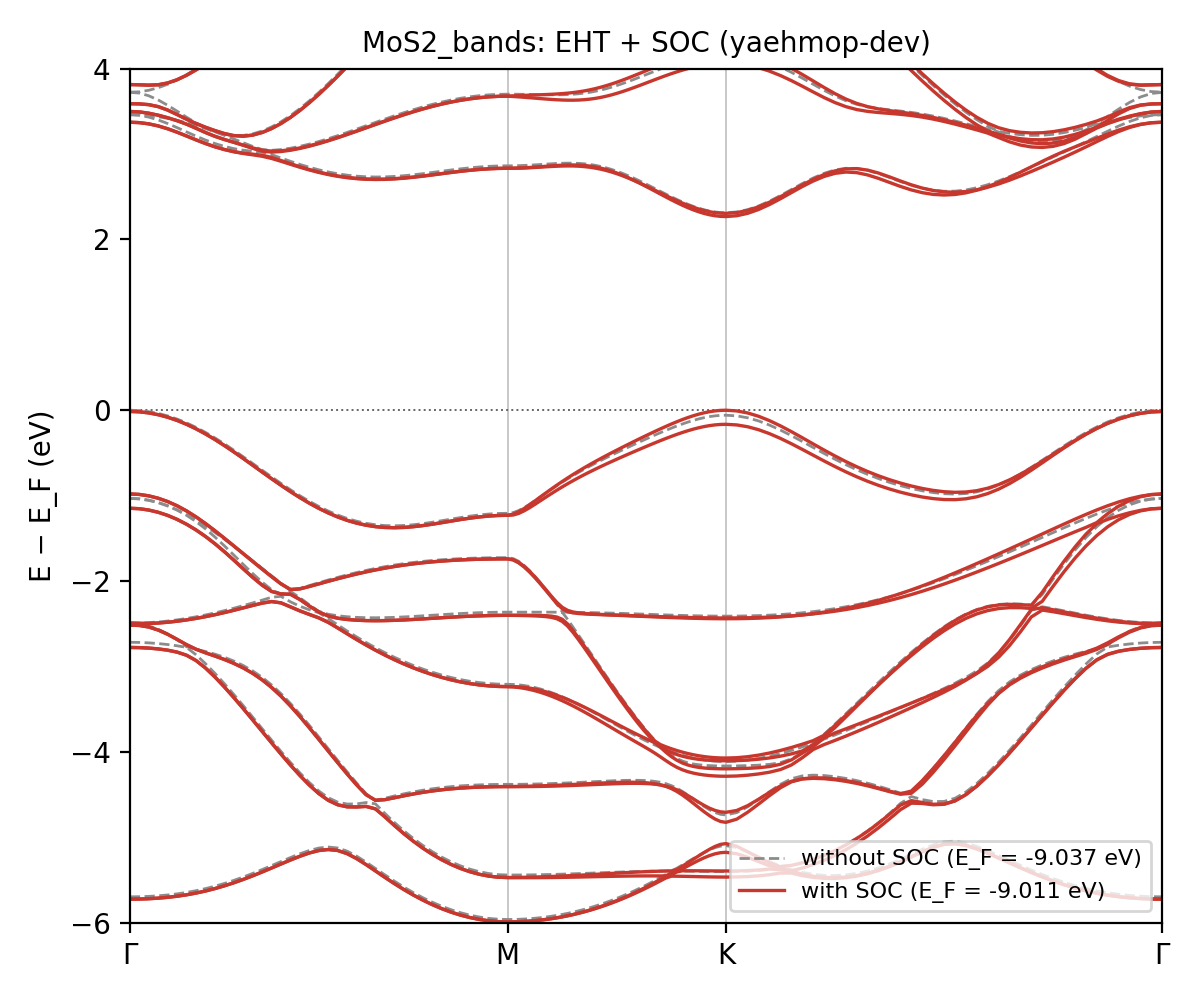
\includegraphics[width=0.62\textwidth]{../new_tests/MoS2_SOC/out/bands_soc.png}
\caption{MoS$_2$ monolayer, EHT bands with (red) and without (gray dashed) SOC, each
relative to its Fermi level (the VBM). The splitting of the valence band at K and of the
conduction bands is visible.}
\label{fig:mos2}
\end{figure}

\subsection{Ferromagnetic bcc Fe, one parameter table per spin channel}

\paragraph{Parametrization.} Each spin channel of a VASP PBE spin-polarized calculation
(magnetic moment 2.238~$\mu_B$) was fitted separately, with its own $H_{ii}$, zetas and
$K$. The $3d$ level of the up (majority) channel is 1.41~eV deeper than that of the down
channel, which is the exchange splitting:
\begin{lstlisting}[style=sh,caption={\file{new\_tests/Fe\_spin/Fe\_up.dat} (top) and \file{Fe\_down.dat} (bottom)}]
FE    26     8     1     4  s -13.819277   1.670952   0.000000   1.000000   0.000000
FE    26     8     1     4  p  -9.457739   1.310866   0.000000   1.000000   0.000000
FE    26     8     2     3  d -16.297432   6.091142   1.923890   1.000000   0.837974
END
FE    26     8     1     4  s -14.099999   1.679093   0.000000   1.000000   0.000000
FE    26     8     1     4  p  -9.602277   1.395172   0.000000   1.000000   0.000000
FE    26     8     2     3  d -14.884268   5.577874   1.827707   1.000000   0.953031
END
\end{lstlisting}
\begin{center}
\begin{tabular}{l c c}
\toprule
 & spin up & spin down \\
\midrule
$K$ (fit) & 1.752806708980162 & 1.7490786283756976 \\
electrons (DFT) & 5.119 & 2.881 \\
\bottomrule
\end{tabular}
\end{center}

\paragraph{Input.} The primitive bcc cell has one atom; atoms 2--4 define the three
lattice vectors. The path is $\Gamma$--H--N--$\Gamma$--P--H, as in the DFT reference, and
average properties and dumps use a $10\times10\times10$ mesh. \texttt{THE CONST} is a
placeholder here, because the command line replaces it in each channel.
\begin{lstlisting}[style=sh,caption={\file{new\_tests/Fe\_spin/Fe\_bands.bind} (the 1000 mesh points are cut)}]
Fe bcc spin polarized

Geometry Crystallographic
4
  1 Fe  0.000000000000  0.000000000000  0.000000000000
  2 Fe  1.000000000000  0.000000000000  0.000000000000
  3 Fe  0.000000000000  1.000000000000  0.000000000000
  4 Fe  0.000000000000  0.000000000000  1.000000000000

Lattice
3
5 5 5
1 2
1 3
1 4

Crystal Spec
2.450119391103 2.450119391103 2.450119391103
109.471220634491 109.471220634491 109.471220634491

THE CONST 1.750000000000

Band
40
6
G    0.000000000000  0.000000000000  0.000000000000
H    0.500000000000 -0.500000000000  0.500000000000
N    0.000000000000  0.000000000000  0.500000000000
G    0.000000000000  0.000000000000  0.000000000000
P    0.250000000000  0.250000000000  0.250000000000
H    0.500000000000 -0.500000000000  0.500000000000

Average Properties

Electrons
8

Dump Hamil
Dump Overlap

K points
1000
 ...
\end{lstlisting}

\paragraph{Run.}
\begin{lstlisting}[style=sh]
cd new_tests/Fe_spin/out
cp ../Fe_bands.bind .
yaehmop --parm-up ../Fe_up.dat --parm-down ../Fe_down.dat \
        --const-up 1.752806708980162 --const-down 1.7490786283756976 \
        --nelec-up 5.119 --nelec-down 2.881 \
        Fe_bands.bind
python3 plot_bands.py --emin -8 --emax 6                      # bands_spin.png
\end{lstlisting}

\paragraph{Outputs.} Two sets of files, \texttt{Fe\_bands\_up.bind.*} and
\texttt{Fe\_bands\_down.bind.*} (\texttt{.band} with 9 bands, \texttt{.HAM}/\texttt{.OV}
$9\times9$ on 1000 $k$ points, \texttt{.out}, \texttt{.status}). The two \texttt{.OV}
files differ because the zetas differ. The header of each \texttt{.out} records the channel:
\begin{lstlisting}[style=sh]
#SPIN_CHANNEL: up
; parameter file of this channel: ../Fe_up.dat
; electrons from the input (both channels): 8.000000
#ELECTRONS_THIS_CHANNEL: 5.119000
; THE CONST of the input (1.750000) replaced by 1.752807 for this channel
#THE_CONST: 1.752807
\end{lstlisting}

\paragraph{Results.} The Fermi levels of the channels are $-14.332$~eV (up) and
$-15.055$~eV (down). The fit had placed the DFT Fermi level at $-14.259$ and $-14.895$~eV;
the small differences come from the $10\times10\times10$ mesh without smearing. The
majority $d$ bands lie below $E_F$ and the minority $d$ bands around and above it, as
expected for a ferromagnet (Fig.~\ref{fig:fe}).

\begin{figure}[H]
\centering
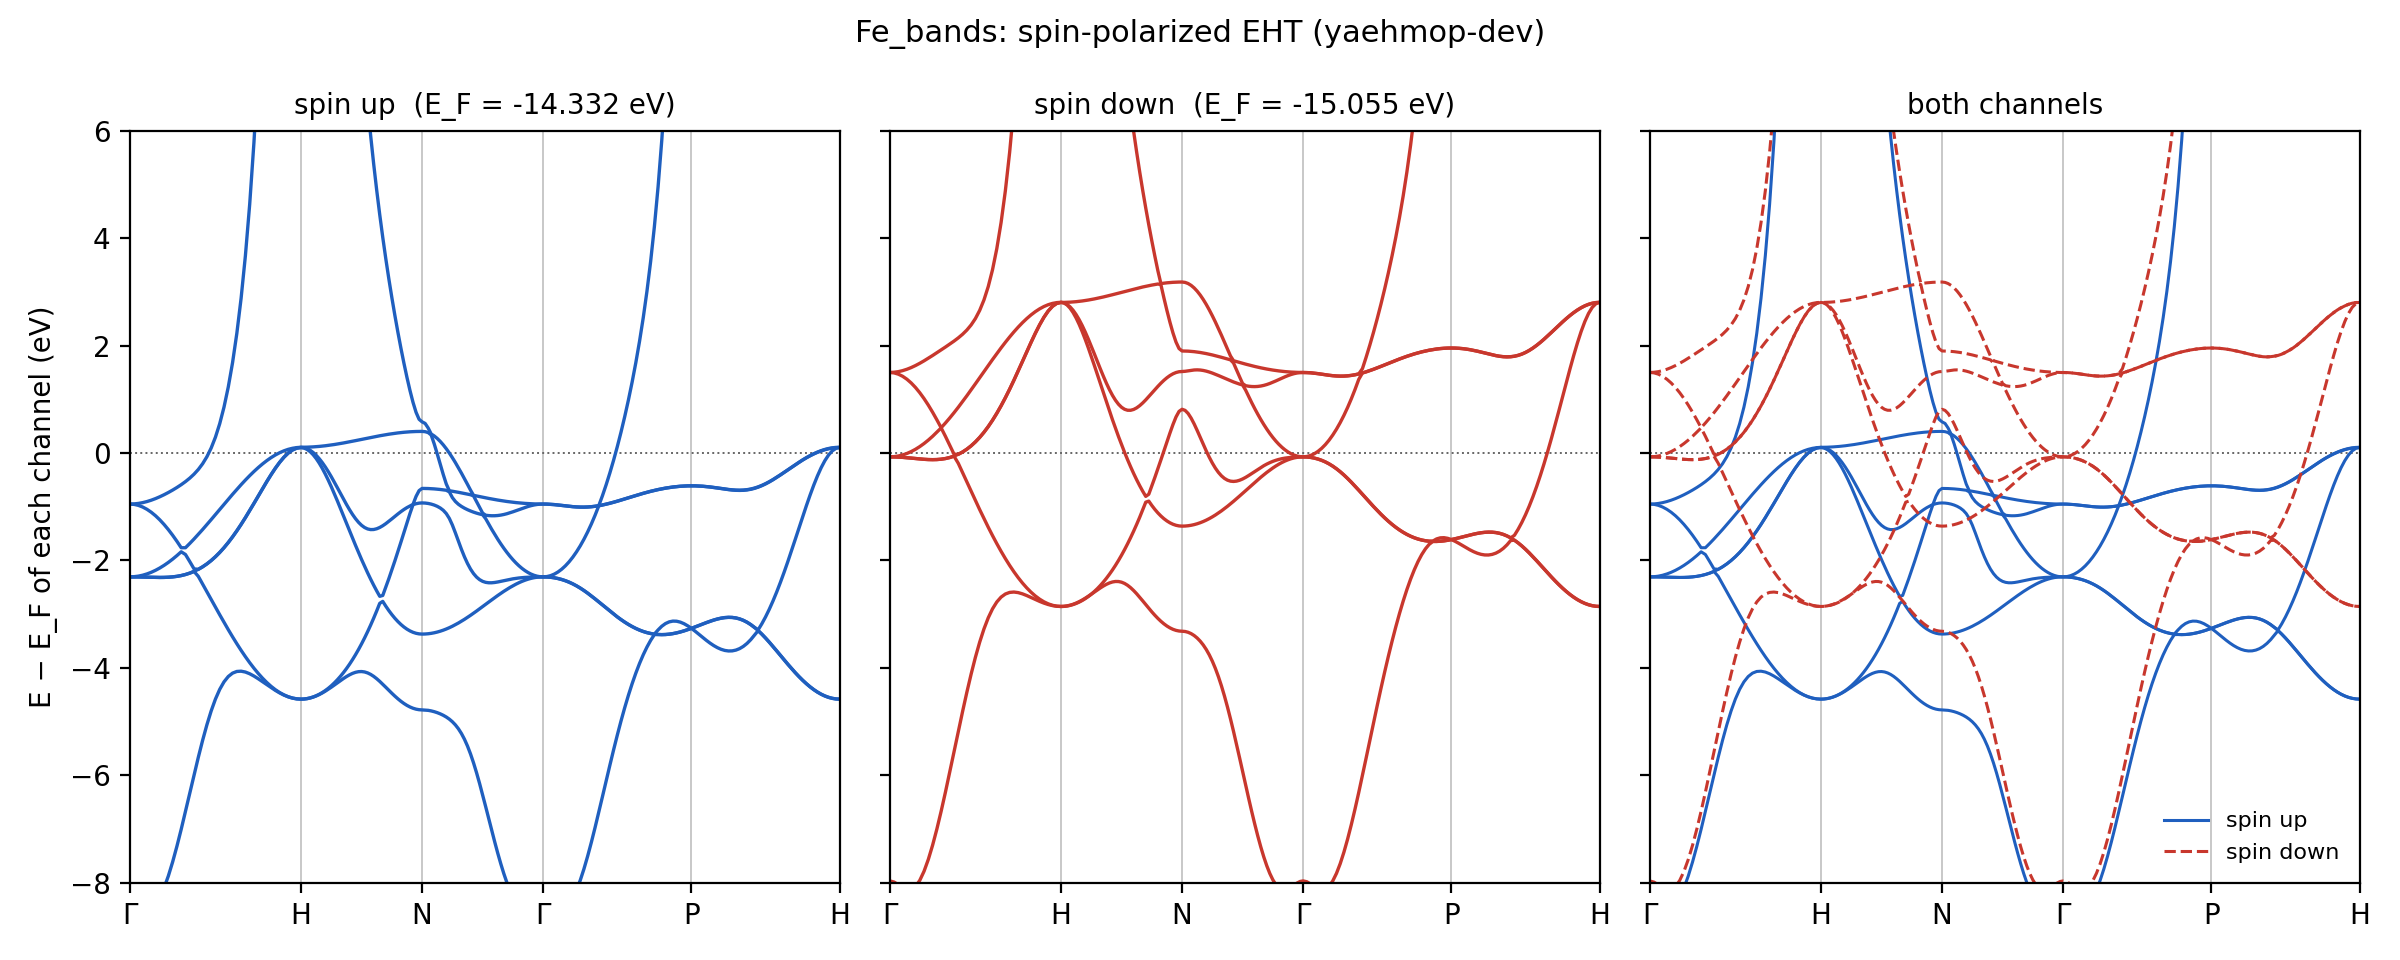
\includegraphics[width=\textwidth]{../new_tests/Fe_spin/out/bands_spin.png}
\caption{bcc Fe, EHT bands of the spin-up and spin-down channels and both together, each
relative to its own Fermi level.}
\label{fig:fe}
\end{figure}

\end{document}
